% !TEX TS-program = pdflatex
% !TEX encoding = UTF-8 Unicode

% This is a simple template for a LaTeX document using the "article" class.
% See "book", "report", "letter" for other types of document.

\documentclass[11pt]{article} % use larger type; default would be 10pt
\usepackage[spanish]{babel}
\usepackage[utf8]{inputenc} % set input encoding (not needed with XeLaTeX)
\usepackage{ctable}
\usepackage{sectsty}
\usepackage[all]{xy}
%%% Examples of Article customizations
% These packages are optional, depending whether you want the features they provide.
% See the LaTeX Companion or other references for full information.
%%% PAGE DIMENSIONS
\usepackage{geometry} % to change the page dimensions
\geometry{a4paper} % or letterpaper (US) or a5paper or....
% \geometry{margin=2in} % for example, change the margins to 2 inches all round
% \geometry{landscape} % set up the page for landscape
%   read geometry.pdf for detailed page layout information
\usepackage[rightcaption]{sidecap}
\usepackage{graphicx} % support the \includegraphics command and options
\usepackage{amsmath}
\usepackage{amsfonts}
% \usepackage[parfill]{parskip} % Activate to begin paragraphs with an empty line rather than an indent

%%% PACKAGES
\usepackage{booktabs} % for much better looking tables
\usepackage{listings}
\usepackage{array} % for better arrays (eg matrices) in maths
\usepackage{paralist} % very flexible & customisable lists (eg. enumerate/itemize, etc.)
\usepackage{verbatim} % adds environment for commenting out blocks of text & for better verbatim
\usepackage{subfig} % make it possible to include more than one captioned figure/table in a single float
% These packages are all incorporated in the memoir class to one degree or another...
\usepackage{amsfonts}
\usepackage{amsmath,amssymb}
\usepackage{graphicx}
\usepackage{listings}
%%% HEADERS & FOOTERS
\usepackage{fancyhdr} % This should be set AFTER setting up the page geometry
\pagestyle{fancy} % options: empty , plain , fancy
\renewcommand{\headrulewidth}{0pt} % customise the layout...
\lhead{}\chead{}\rhead{}
\lfoot{}\cfoot{\thepage}\rfoot{}
\usepackage[T1]{fontenc}
%%% SECTION TITLE APPEARANCE
\usepackage{sectsty}
\allsectionsfont{\sffamily\mdseries\upshape} % (See the fntguide.pdf for font help)
% (This matches ConTeXt defaults)
\usepackage[ruled,vlined]{algorithm2e}
%%% ToC (table of contents) APPEARANCE
\usepackage[nottoc,notlof,notlot]{tocbibind} % Put the bibliography in the ToC
\usepackage[titles,subfigure]{tocloft} % Alter the style of the Table of Contents
\renewcommand{\cftsecfont}{\rmfamily\mdseries\upshape}
\renewcommand{\cftsecpagefont}{\rmfamily\mdseries\upshape} % No bold!

%%% END Article customizations
% ==========================
% = Matemáticas y teoremas =
% ==========================
\usepackage[]{amsmath}
\usepackage[]{amsthm}
\usepackage[]{mathtools}
\usepackage[]{bm}
\usepackage[]{thmtools}
\newcommand{\marcador}{\vrule height 10pt depth 2pt width 2pt \hskip .5em\relax}
\newcommand{\cabeceraespecial}{%
	
	\normalfont\bfseries}
\declaretheoremstyle[
spaceabove=\medskipamount,
spacebelow=\medskipamount,
headfont=\cabeceraespecial\marcador,
notefont=\cabeceraespecial,
notebraces={(}{)},
bodyfont=\normalfont\itshape,
postheadspace=1em,
numberwithin=section,
headindent=0pt,
headpunct={.}
]{importante}
\declaretheoremstyle[
spaceabove=\medskipamount,
spacebelow=\medskipamount,
headfont=\normalfont\itshape,
notefont=\normalfont,
notebraces={(}{)},
bodyfont=\normalfont,
postheadspace=1em,
numberwithin=section,
headindent=0pt,
headpunct={.}
]{normal}
% Los nombres de los enunciados. Añade los que necesites.
\declaretheorem[name=Observaci\'on, style=normal]{remark}

\declaretheorem[name=Corolario, style=normal]{corollary}

\declaretheorem[name=Proposici\'on, style=normal]{proposition}

\declaretheorem[name=Lema, style=normal]{lemma}

\declaretheorem[name=Ejemplo , style=definition, numberwithin=section]{ejemplo}


\declaretheorem[name=Teorema, style=importante]{theorem}

\declaretheorem[name=Definici\'on, style=importante]{definition}



%%% The "real" document content comes below...
\title{Análisis de sentimientos multimodal}
\author{Sara Olías Zapico}

\begin{document}
	\maketitle
\renewcommand{\refname}{Bibliografía}

\tableofcontents

\newpage

\section{Recopilación de datos}

Lo primero que debemos hacer para comenzar el desarrollo del trabajo es recoger el histórico de datos de BTC necesario. Para ello hemos utilizado la librería \textit{ccxt} de python. Esta librería contiene una colección de extracciones de diferentes criptomonedas. Para nuestro trabajo hemos extraido las correspondientes con BTC/USDT. 


Hemos realizado dos extracciones para las diferentes pruebas: en la primera se obtiene una fila por día desde el 17 de Agosto de 2017; en la segunda, se obtiene una fila por hora desde el 17 de Agosto de 2017 a las 04:00. En ambos casos las columnas extraidas son: valor de cierre, fecha, valor máximo alcanzado en ese periodo, valor mínimo y volumen medio por transacción.


Como estos indicadores eran insuficientes, hemos añadido nuevos indicadores a nuestro conjunto inicial y, de esta manera, hemos creado tres conjuntos de datos para poder comparar como cambia el rendimiento de nuestros modelos conforme se aumenta el número de indicadores.

\textbf{\begin{center}
		CONJUNTO DE DATOS 1
\end{center}}

A las columnas iniciales le añadimos las siguientes:

\begin{itemize}
	\item \textbf{Anterior:} precio de cierre del periodo anterior.
	
	\item \textbf{Diferencia:} diferencia de precio de cierre entre el periodo anterior y el actual.
	
	\item \textbf{Anterior-1:} precio de cierre de dos periodos atrás.
	
	\item \textbf{Diferencia-1:} diferencia de precio de cierre entre el periodo anterior y el de antes de éste.
	
	\item \textbf{Subida:} tiene el valor 1 si del periodo anterior al actual el precio de cierre ha subido, 0 si ha bajado.
	
	\item \textbf{Subida-1:} tiene el valor 1 si de dos periodos atrás al anterior el precio de cierre ha subido, 0 si ha bajado.
	
\end{itemize}

Al añadir estas colunmas, algunos datos se quedaban en blanco, ya que no teniamos los datos de los dias anteriores de las dos primeras filas; por lo que hemos tenido que eliminar estas filas. Adjuntamos una extracción del primer conjunto de datos creado:

\newpage

\begin{center}
	\begin{figure}[htb]
		\centering
		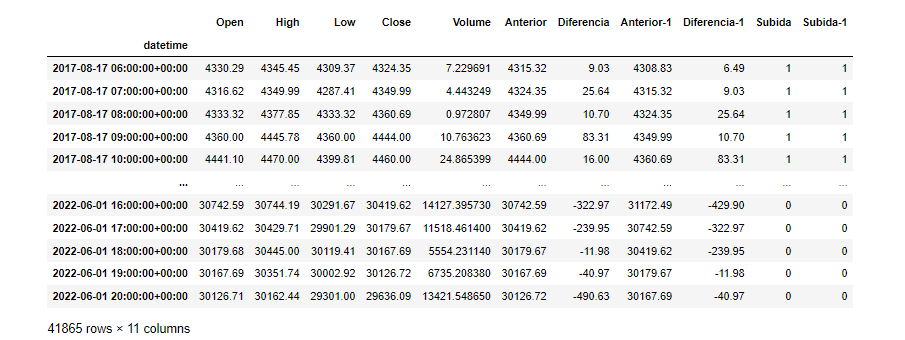
\includegraphics[scale = 0.6]{Datos1-ejemplo.png}
		\caption{Extracción del conjunto de datos 1.}
	\end{figure}
\end{center}


\textbf{\begin{center}
		CONJUNTO DE DATOS 2
\end{center}}


Para crear este conjunto de datos, vamos a agregar al conjunto de datos anterior los siguientes indicadores:

\begin{itemize}
	
	\item \textbf{Precio Medio Ponderado por Volumen(VWAP):} este indicador nos muestra la relacion que hay entre el precio del BTC y el volumen de las operaciones diarias.
	
	\item \textbf{SMA10:} una media móvil simple (o aritmética) es una media móvil aritmética calculada sumando los elementos de una serie temporal y dividiendo este total por el número de períodos de tiempo. Media SMA con 10 periodos anteriores.

	\item \textbf{SMA20:} Media SMA con 20 periodos anteriores.

	\item \textbf{SMA55:} Media SMA con 55 periodos anteriores.

	\item \textbf{EMA10:} las medias móviles exponenciales dan más peso a los períodos más recientes. Esto los hace más seguras que la SMA y por lo tanto pueden ser usadas para crear una mejor estrategia de trading con medias móviles. Media EMA con 10 periodos anteriores

	\item \textbf{EMA20:} Media EMA con 20 periodos anteriores.

	\item \textbf{EMA55:} Media EMA con 55 periodos anteriores.

	\item \textbf{VMA10:} sirven para frenar el promedio cuando los precios están en el período de consolidación, para evitar señales malas y acelerar el promedio cuando el mercado está en tendencia para aprovechar al máximo los precios en tendencia.  Media VMA con 20 periodos anteriores.

	\item \textbf{VMA20:} Media VMA con 20 periodos anteriores.

	\item \textbf{VMA55:} Media VMA con 20 periodos anteriores.
	
\end{itemize}

\begin{center}
	\begin{figure}[htb]
		\centering
		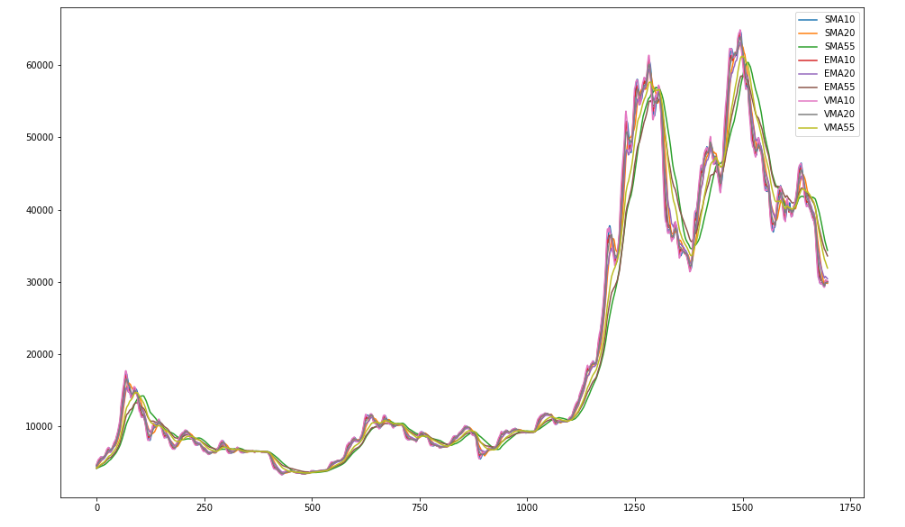
\includegraphics[scale = 0.6]{mediasmoviles.png}
		\caption{Representación grafica de las medias moviles para el conjunto de datos por días.}
	\end{figure}
\end{center}


Como podemos ver, en el conjunto de datos 2 hemos añadido varias medias móviles. Las medias móviles son uno de los indicadores técnicos más conocidos ya que son fáciles de usar. En estadística, las medias móviles son unas medidas que van tomando los datos referentes a un periodo temporal definido. Conforme se va avanzando en el tiempo, los datos a evaluar también avanzan, ajustándose y actualizándose de forma sucesiva. 


Cuando hablamos de series temporales, las medias móviles son muy útiles. Cuanto mayor sea el periodo, la media móvil es más lenta en dar señales, pero las señales serán mas fiables; es por ello que las medias móviles con periodos mas altos, van a ser más útiles para los datos por horas, ya que tenemos mas registros.


Hay varios tipos de medias móviles, en nuestro caso vamos a estudiar la media móvil aritmética (\textit{SMA}), la media móvil exponencial (\textit{EMA}) y la media móvil variable (\textit{VMA}). Veamos cada una de ellas por separado \cite{mmovil}:

\begin{itemize}
	\item[$-$] \textbf{Media Móvil Simple o Aritmética (SMA)}:

Una media móvil simple (o aritmética) es una media móvil aritmética calculada sumando los elementos de una serie temporal y dividiendo este total por el número de períodos de tiempo. Este es el tipo mas simple de todos los promedios móviles. En esta media, los pesos son los mismos para todos los elementos (si tenemos un periodo n, el peso asociado será $\frac{1}{n}$. Generalmente esta media es útil para identificar la dirección de la tendencia.

$$
SMA = \dfrac{(\text{ Suma de los n últimos datos })} {(\text{ Número total de periodos })}
$$

	
	\item[$-$] \textbf{Media Móvil Exponencial (EMA)}:	
Cuando hay picos en el precio a estudiar, las medias móviles simples no funcionan muy bien. Las medias móviles exponenciales dan más peso a los periodos más actuales, su cálculo es:



\begin{align}
	\text{EMA actual }&  = \text{ [Precio de cierre – EMA (día anterior)] $*$ multiplicador + EMA (día anterior) }  \nonumber \\
	 &donde  \nonumber \\
	Multiplicador  &=  2 ÷ (cantidad de períodos seleccionados + 1)] \nonumber
\end{align}

La media móvil exponencial es más rápida en reaccionar que la SMA, esto se debe a que cada término del periodo de la media móvil tiene un peso exponencialmente mayor que el término anterior.

	
	\item[$-$] \textbf{Meda móvil variable (VMA)} \cite{vma}:
	
La \textit{VMA} es una media móvil ponderada exponencialmente, para ello se utiliza un Índice de Volatilidad (\textit{VI}) que mide la rapidez o lentitud con la que los precios cambian a lo largo del tiempo. 

El propósito principal del \textit{VMA} es frenar la media cuando los precios se están consolidando y acelerar esta media cuando los precios están en tendencia.

\begin{align}
	\text{VMA }&  = (\alpha * VI * \text{Precio de cierre})+(1-(\alpha*VI))*VMA[1] \nonumber \\
	 \alpha &  = \frac{2}{(N+1)} \nonumber \\
	\text{N }&  = \text{periodo sobre el que se realiza la media} \nonumber \\
	\text{VMA[1] }&  = \text{VMA del periodo anterior} \nonumber 
\end{align}


\end{itemize}

Podemos ver las principales diferencias de ajuste en esta gráfica, creada a partir de las medias de los datos de un día (los últimos 100 registros):

\begin{center}
	\begin{figure}[htb]
		\centering
		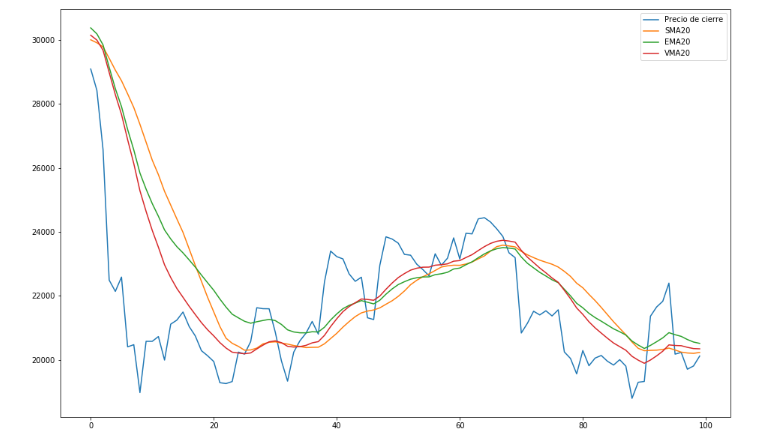
\includegraphics[scale = 0.6]{medias100.png}
		\caption{Representacion SMA20, EMA20 y VMA20 frente al precio de cierre}
	\end{figure}
\end{center}


\newpage

\textbf{\begin{center}
		CONJUNTO DE DATOS 3
\end{center}}


Para este tercer conjunto, vamos a añadir al conjunto de datos 2, varios indicadores:

\begin{itemize}
	\item \textbf{Indicador MACD (Moving Average Convergene Divergence) \cite{macd} }:

Mide la convergencia y divergencia en el tiempo de dos medias móviles del precio de un activo. En otras palabras el MACD señala, en cada momento, la separación entre el valor de dos medias móviles con diferente período de cálculo. Para el cálculo del MACD utilizamos la media movil exponencial (EMA), primero calculada en un periodo corto y después en un periodo medio, y calulamos la diferencia entre ambas. Normalmente, para la media corta se emplean 12 períodos y, para la otra media, 26 períodos. (MACD = EMA (12) – EMA (26)).

Después de obtener el MACD, se calcula, a su vez, su media móvil exponencial. Para realizar este cálculo se suele emplear una media de 9 períodos. Esta media móvil se denomina Señal. El histograma MACD representa la diferencia entre MACD y su EMA de 9 días, la línea de señal.

\begin{center}
	\begin{figure}[htb]
		\centering
		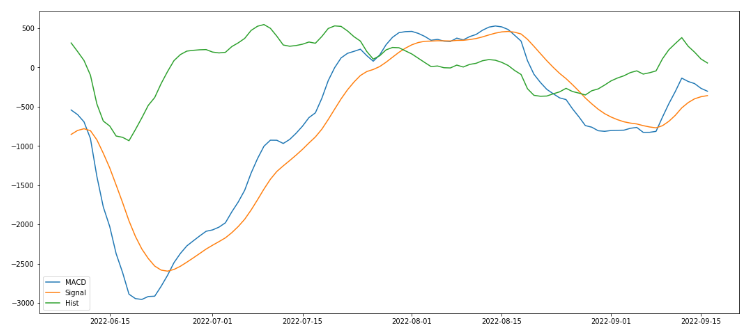
\includegraphics[scale = 0.6]{macd.png}
		\caption{Representacion MACD}
	\end{figure}
\end{center}

\newpage

	\item \textbf{Indicador KDJ }:
	
Las líneas \textit{K} y \textit{D} del oscilador estocástico (señalan una tendencia inminente cuando ocurren divergencias alcistas y bajistas.) y la \textit{J} muestra la divergencia del valor \textit{D} de la \textit{K}. Gráficamente:

\begin{center}
	\begin{figure}[htb]
		\centering
		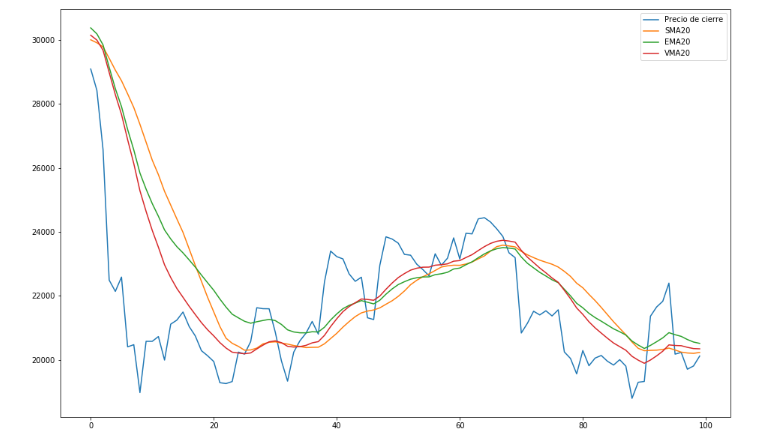
\includegraphics[scale = 0.6]{medias100.png}
		\caption{Representacion KDJ}
	\end{figure}
\end{center}
	

	\item \textbf{Bandas de Bollinger } \cite{bollinger}:

El indiador bandas de Bollinger utiliza una medida estadística conocida como la desviación estándar para determinar dónde podría tener lugar un posible nivel de soporte o resistencia. Estas bandas se conforman por dos lineas, una por encima y otra por debajo de una media central.

La media central es una SMA de periodo N; la banda superior se dibuja en X desviaciones estándar por encima de la media anterior y la banda inferior, se dibuja en X desviaciones estándar por debajo de la media. Nosotros hemos escogido hacer la media SMA con 20 periodos y con una desviación estándar multiplicada por 2. Para estos parámetros, las estadísticas muestran que el 95$\textdiscount$ del precio debe permanecer dentro de las Bandas de Bollinger.

\begin{center}
	\begin{figure}[htb]
		\centering
		\includegraphics[scale = 0.6]{bollinger.png}
		\caption{Representacion Bandas de Bollinger}
	\end{figure}
\end{center}
	
	
	\item \textbf{RSI(Relative Strength Index) }:	

es un indicador de tipo oscilador que refleja la fuerza relativa de los movimientos alcistas, en comparación con los movimientos bajistas. Es utilizado por los traders para medir la fuerza de una tendencia e identificar señales de fin de tendencia. El oscilador se mueve entre los valores 0 y 100. Si el indicador esta por debajo de 30 se dice que está en \textit{sobreventa}, y el precio tiende a subir. Cuando se encuentra por encima de 70, decimos que esta en \textit{sobrecompra} y que el precio tenderá a bajar.


\begin{center}
	\begin{figure}[htb]
		\centering
		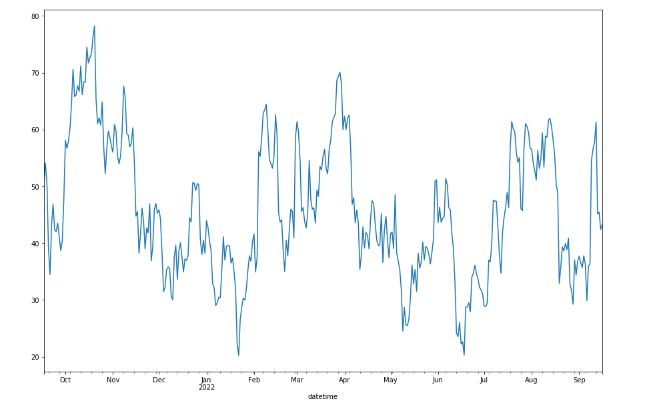
\includegraphics[width=12cm, height=5cm]{RSI.png}
		\caption{Representacion RSI}
	\end{figure}
\end{center}

\newpage

	\item \textbf{Estocastico } \cite{estocastico}:
	
significa la comparación realizada por el indicador estocástico entre el precio de cierre actual y sus precios de cierre anteriores durante un período elegido. El Oscilador Estocástico se mide usando las líneas K y D, que se definen:

$$
K = 100 [(C -Ln)/(Hn-Ln)] \text{ ;  }D = \text{es la media móvil de K en N periodos}
$$	
donde  C es el precio de cierre actual; Ln es el precio más bajo durante los últimos "n" periodos; Hn es el precio más alto durante las últimos "n" periodos.	

Para interpretarlo sabemos que: si el precio de cierre actual es cercano al precio más alto (Hn) del período en cuestión, el estocástico estará cerca del 100 $\textdiscount$ ; si el precio de cierre actual está cerca del precio más bajo (Bn) del período relevante, el estocástico estará cerca del 0 $\textdiscount$.

\begin{center}
	\begin{figure}[htb]
		\centering
		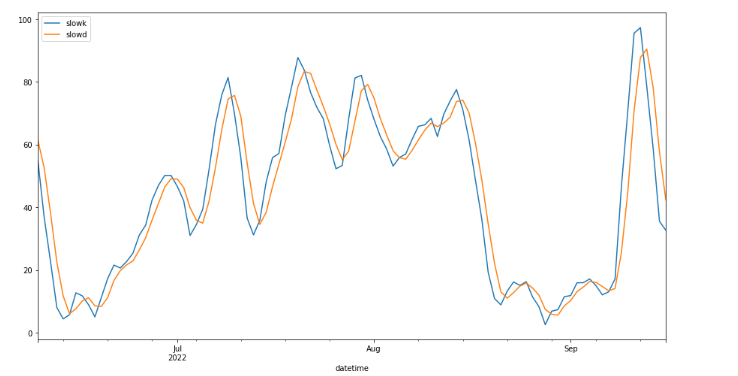
\includegraphics[width=12cm, height=5cm]{estocas.png}
		\caption{Representacion indicador estocástico}
	\end{figure}
\end{center}

\newpage

	\item \textbf{Indicador ATR (Average True Range) } \cite{atr}:	
	
calcula la volatilidad existente en el periodo actual. El ATR sube o baja cuando el activo tiene mas o menos volatilidad; es decir, cuando el valor de ATR es alto, hay una alta volatilidad y unos valores bajos indican una estabilidad en los precios.

Para calcularlo, llamamos TR a el valor más alto de entre: el maximo menos el mínimo, el maximo menos el cierre del periodo anterior y el minimo menos el cierre del periodo anterior. Una vez tenemos este valor, calculamos lo siguiente:
$$
ATR = (\text{ATR anterior}*(n-1)+\text{TR(periodo actual)})/n
$$

donde \textit{n} indica el periodo en el que calculamos esta media.
		

\begin{center}
	\begin{figure}[htb]
		\centering
		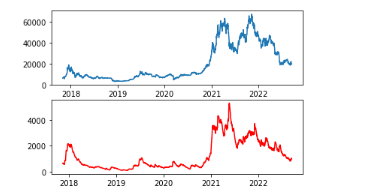
\includegraphics[width=12cm, height=3.5cm]{atr.png}
		\caption{Comparación precio de cierre (arriba) con valores del indicador ATR (abajo)}
	\end{figure}
\end{center}


	\item \textbf{Funciones de Reconocimiento de patrones (BELTHOLD) } :	

al ingresar los datos de apertura, máximo, mínimo y cierre de la acción en estudio la función seleccionada retornara uno de tres posibles valores enteros, 0 cuando no reconoce patrón, 100 cuando reconoce un patrón alcista y -100 cuando reconoce un patrón bajista.

\begin{center}
	\begin{figure}[htb]
		\centering
		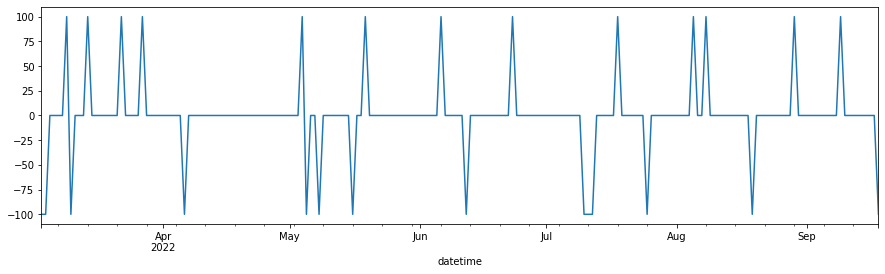
\includegraphics[width=12cm, height=3.5cm]{belthold.png}
		\caption{Representacion BELTHOLD}
	\end{figure}
\end{center}


\end{itemize}


\newpage
\section{Estudio de la correlación de las variables}

El estudio de la correlación nos proporciona información sobre la fuerza de la relación que hay entre las variables. Existe la correlación positiva y negativa. La positiva nos indica que las variables se mueven en la misma dirección, cuando una aumenta, la otra también lo hace. La correlación negativa ocurre cuando se mueven en direcciones opuestas, si una aumenta, la otra disminuye. 

Para estudiar la correlación que existe entre todas las variables vamos a calcular el coeficiente de correlación de Pearson y representarlo gráficamente en un mapa de correlación(\ref{imcorr}).









\begin{center}
	\begin{figure}[htb]
		\centering
		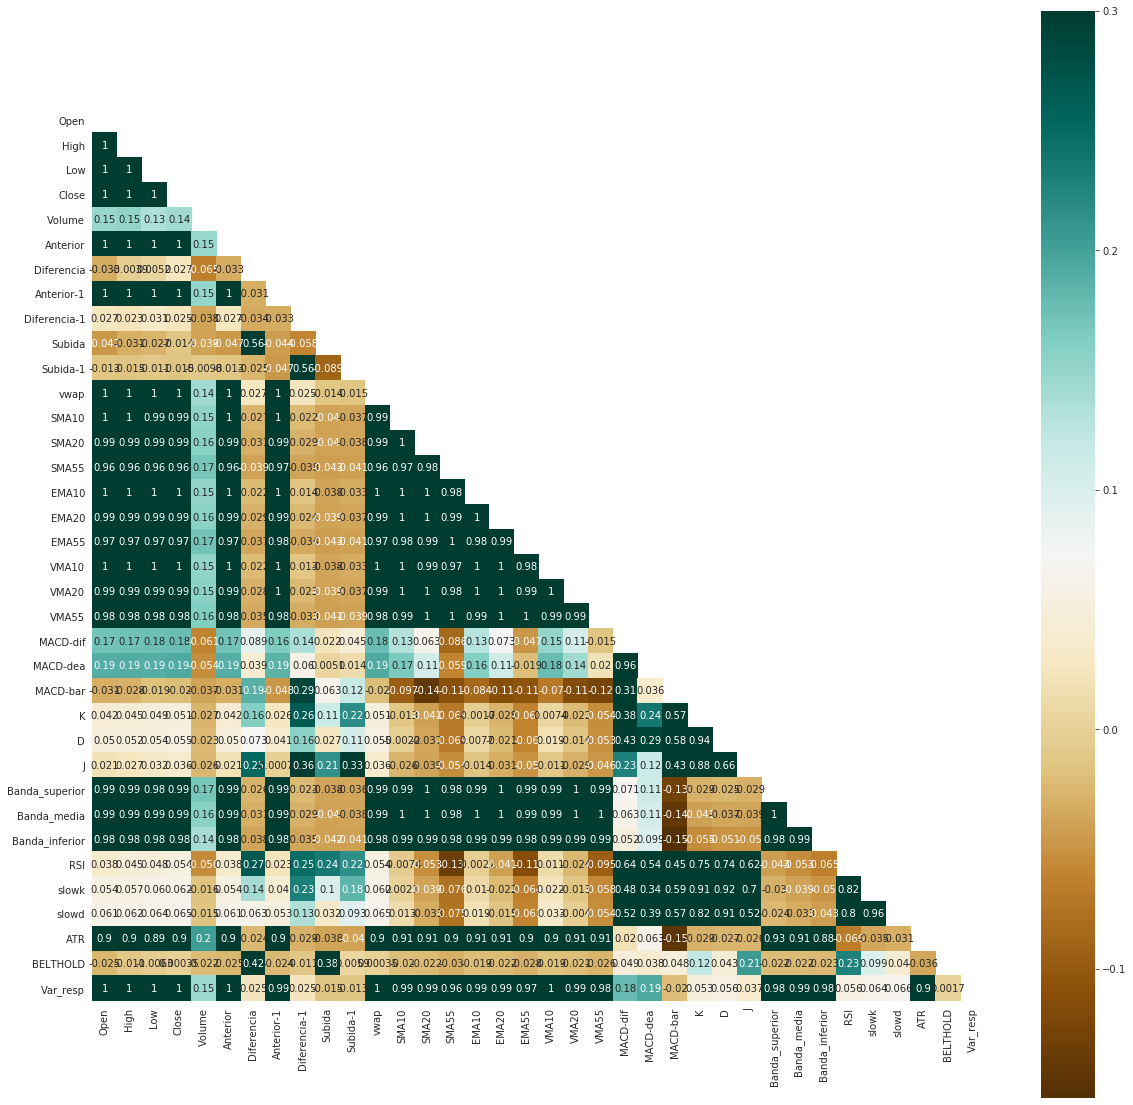
\includegraphics[scale = 0.35]{medcor.png}
		\caption{Mapa de calor para el conjunto de datos 1.}
		\label{imcorr}
	\end{figure}
\end{center}




El coeficiente de correlación de Pearson entre dos variables, X e Y, se calcula utilizando la siguiente fórmula:
$$
Corr(X,Y) = \dfrac{\sum(x_i-\bar{x}) (y_i - \bar{y}) } 
{\sqrt{   \sum(x_i-\bar{x})^2 \sum (y_i - \bar{y})^2         }}
$$


Donde: $\bar{x}$ es el valor medio de x, $\bar{y}$ es el valor medio de y, $x_i$ es el i-ésimo valor de x e $y_i$ es el i-ésmo valor de y.

Los valores de correlación tan entre -1 y 1; si el valor es 1 hay una correlación positiva, si el valor es -1, hay una correlación positiva y, si es 0 indica que no hay correlación entre las variables.



Si nos fijamos en el primer conjunto de datos, podemos observar que tienen muy buena correlacion las variables Open, Hight,Low, Close, Anterior y Anterior-1; tanto entre ellas como con la variable respuesta. 

Para el segundo conjunto, vemos que todas las medias móviles que hemos añadido tienen una correlación bastante alta, por lo que podemos suponer que este conjunto va a funcionar mejor que el primero.

Por último, en el tercer conjunto, la correlación no es tan alta, parece que el indicador que más aporta al resultado de la variable respuesta son las Bandas de Bollinger.
























\newpage

\begin{thebibliography}{999999}
	
	\bibitem{mmovil} "\textit{Introduction to Moving Averages For Day Trading}", mayo 2022. Nick,P. Disponible: \textit{https://bullsonwallstreet.com/moving-averages-day-trading/}
	
	\bibitem{vma} "\textit{Variable Moving Average – Trading Strategy Backtest}", agosto 2022. Oddmund Groette. Disponible: \textit{https://www.quantifiedstrategies.com/variable-moving-average/}
	
	\bibitem{macd} "\textit{Estrategias de trading MACD}". AVATRADE INTERNATIONAL. Disponible: \textit{https://www.avatrade.es/educacion/professional-trading-strategies/macd-trading-strategies/}
	
	\bibitem{bollinger} "\textit{Las bandas de Bollinger}", 2006. John Bollinger . \textit{Visual Chart Group}. 
	
	\bibitem{estocastico} "\textit{El Indicador Estocástico en profundidad}", 11 julio 2022. Admirals Markets. Disponible: \textit{https://admiralmarkets.com/es/education/articles/forex-indicators/indicador-estocastico?utm$\_$source=google$\&$utm$\_$medium=cpc$\&$utm$\_$campaign=ES$\_$E	
	S$\_$performance$\_$max$\_$new$\&$utm$\_$term=$\&$gclid=EAIaIQobChMIm-bP$\_$sKy9wIV1vZRCh0T1gvKEAAYAiAAEgIzZfD$\_$BwE}	
	
	\bibitem{atr} "\textit{¿Qué es el Average True Range (ATR) y cómo utilizarlo?}", 28 de Enero 2021. Luis Ángel Hernandez. Disponible: \textit{https://www.rankia.com/blog/bolsa-desde-cero/3529085-que-average-true-range-atr-como-utilizarlo}		
	
\end{thebibliography}


\end{document}
